\section{Methodology}

\begin{figure}[h]
  \centering
  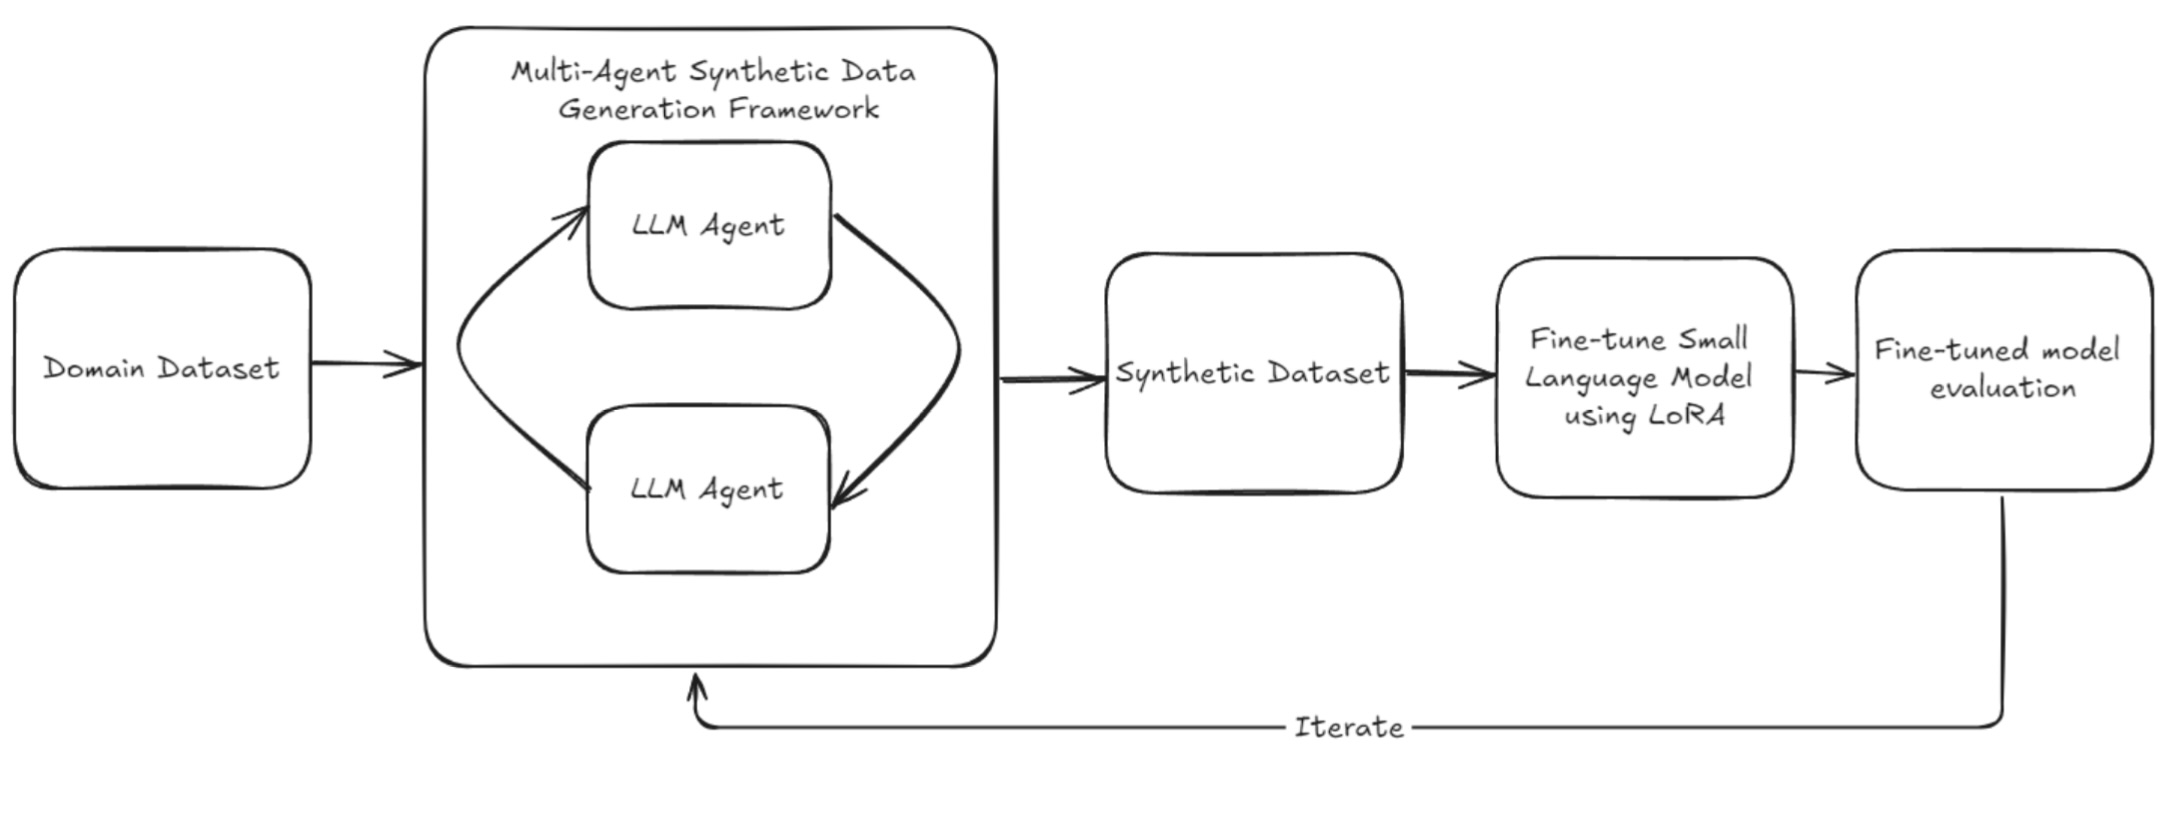
\includegraphics[width=1\textwidth]{methodology.jpg}
  \caption{An overview of our methodology. Given a user-provided dataset, our
framework will employ co-operating agents to create a synthetic dataset that is
used to fine-tune a SLM for downstream tasks. The resulting model can be further
fine-tuned with additional synthetic data derived from the domain dataset.}
\end{figure}

% For our domain datasets that will be used as the seed data, we are still
% currently exploring datasets that can be used. Current ideas include research
% papers, company financial data, technical reports and manuals, or company
% specific FAQ data.
We will develop a multi-agent framework that uses small language models such as
Llama-3.1-8B, Llama-3.2-3B, Qwen2.5-7B. In our approach, these agents generate a
diverse set of synthetic data such that models fine-tuned on this data yield
better performance on their domain-specific task. For example, for an LLM
designed to perform as a chatbot for a particular company, a ``Question-Answer''
agent could generate question-answer pairs from the domain dataset. Additional
agents could further mutate these pairs to increase diversity of the dataset,
for example, a ``Distractor'' agent could modify the question to include
irrelevant details.

Our immediate goal will be to develop agents for LLMs that specialise in
question answering tasks, similar to that of a traditional chatbot. Time
permitting, we may investigate the development of agents to generate synthetic
data to reduce hallucinations.

Our framework will use the synthetic data to fine-tune LoRA adapters on the base
model chosen. Since this will be an iterative process, we may also choose to
perform a full supervised fine-tune of the model depending on resource
limitations.

\subsection{Challenges}

One of the challenges we foresee may be overfitting on the fine-tuned model and
the model's inability to generalise to different writing styles and formats. We
plan to mitigate this by increasing the diversity of our generated data. Another
challenge is hallucination: previous research has shown that fine-tuning LLMs
with new factual information increases their tendency to hallucinate
\citep{gekhman_does_2024}. However, because we consider applications where the
questions posed to the LLMs are related to data in the fine-tuning dataset, it's
possible that this effect will be reduced (as opposed to questions unrelated to
the domain, where a clear effect has already been observed in existing
literature).
